\apendice{Documentación de usuario}

\section{Introducción}
Esta apendice contiene la información orientada a los usuarios, tanto profesores como alumnos, para el correcto acceso y manejo de la plataforma.

\section{Requisitos de usuarios}

\subsection{Requisitos de profesores}
Para poder dar un uso adecuado a la aplicación se recomienda a los profesores la instalación de \textbf{Jupyter Notebooks} y \textbf{Nbgrader} en su entorno de trabajo personal para la creación de tareas. Estos pueden prescindir de ello ya que la plataforma permite edición de tareas desde esta pero, en el caso de que requieran visualizar las entregas de los alumnos descargadas, necesitaran de al menos \textbf{Jupyter Notebooks} para hacerlo.

En cuanto al acceso a la plataforma no se requiere de ningún requisito previo debido a la naturaleza web de esta. Estos podrán acceder a ella en el siguiente enlace \url{http://3.89.140.10/}.

\subsection{Requisitos de alumnos}
En lo que a los alumnos respecta, estos deberán tener instalado de forma obligatoria \textbf{Jupyter Notebooks} en su entorno de trabajo para la resolución de tareas.

Como se ha mencionado previamente, no se requiere de ningún requisito previo en cuanto al acceso a la plataforma web. Estos podrán acceder a ella en el siguiente enlace \url{http://3.89.140.10/}.

\section{Instalación}
Al tratarse de una plataforma web no es necesaria ninguna instalción previa para el acceso a esta. Alumnos y profesores podrán acceder a la plataforma en el siguiente enlace: \url{http://3.89.140.10/}.



\section{Manual del profesor}
A continuación se explicará el manejo de la plataforma orientado a los profesores:

\subsection{1 Acceso a la Plataforma}
El acceso a la plataforma es realizado a través del siguiente enlace: \url{http://3.89.140.10/} el cual nos lleva a la página inicial de esta.

\begin{figure}[H]
    \centering
    
\includegraphics[width=\textwidth]{img/imgs-memoria/Landing.PNG}
    \caption{Página Inicial}
\end{figure}

\subsection{2 Inicio de Sesión}
El proceso de inicio de sesión contiene los siguientes paso:
\begin{itemize}
\tightlist
    \item Una vez accedido a la Página incial hacer click en el botón \textbf{Acceder} lo cual nos llevará a la página de inicio de sesión:
        \begin{figure}[H]
        \centering
        
\includegraphics[width=\textwidth]{img/imgs-memoria/InicioSesion.PNG}
        \caption{Pagina Inicio de sesión}
        \end{figure}
    \item Introducir los credenciales de inicio de sesión y hacer click en el botón \textbf{Login}. Han sido incluido en el fichero README del repositorio los credenciales de acceso de los 5 profesores definidos incialmente para la aplicación.
    \item Si los credenciales son correctos será llevado a la página principal del profesor:
        \begin{figure}[H]
        \centering
        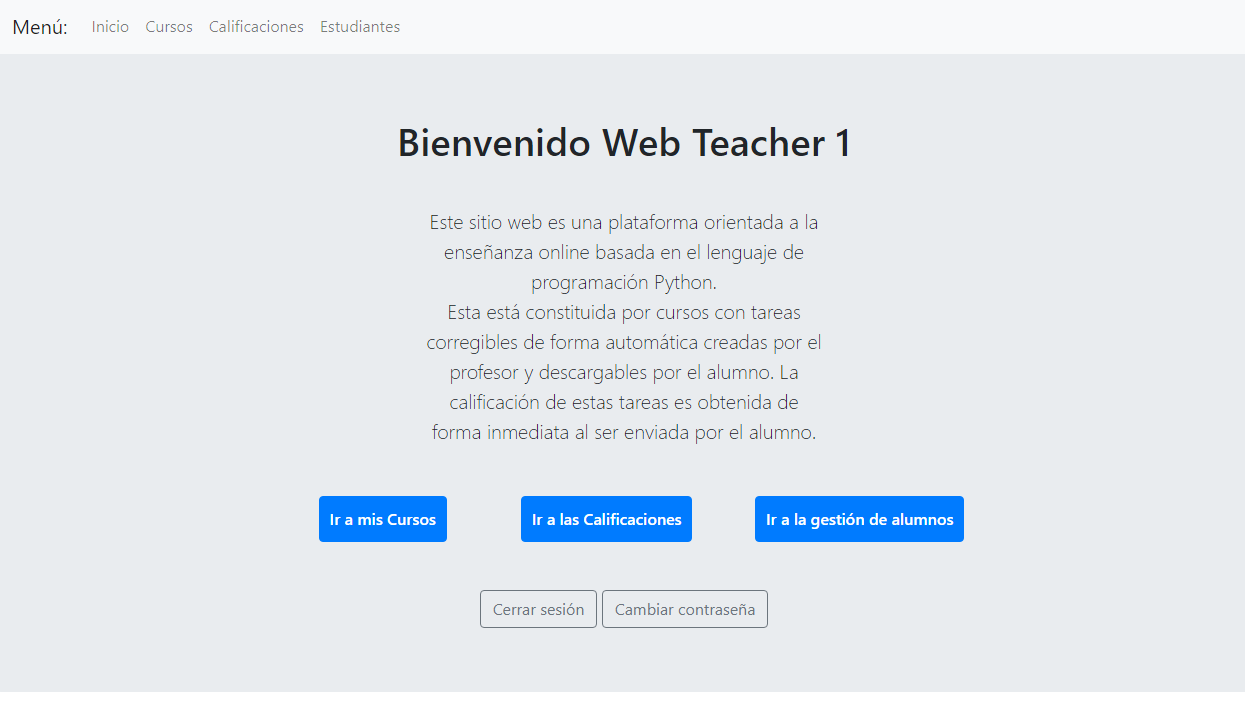
\includegraphics[width=\textwidth]{img/imgs-memoria/TeacherMain.PNG}
        \caption{Página Principal Profesor}
        \label{PagProfesor}
        \end{figure}
\end{itemize}


\subsection{3 Gestión de Cursos}
Para ir a la página de gestión de cursos del profesor se ha de hacer click en el botón \textbf{Ir a mis Cursos} de la \textbf{Página Principal del Profesor}(\ref{PagProfesor}) o en el botón \textbf{Cursos} de la barra navegacional superior. Esto nos llevaría a la página de gestión de cursos en la que se encuentran todos los cursos creados por este profesor:
\begin{figure}[H]
\centering
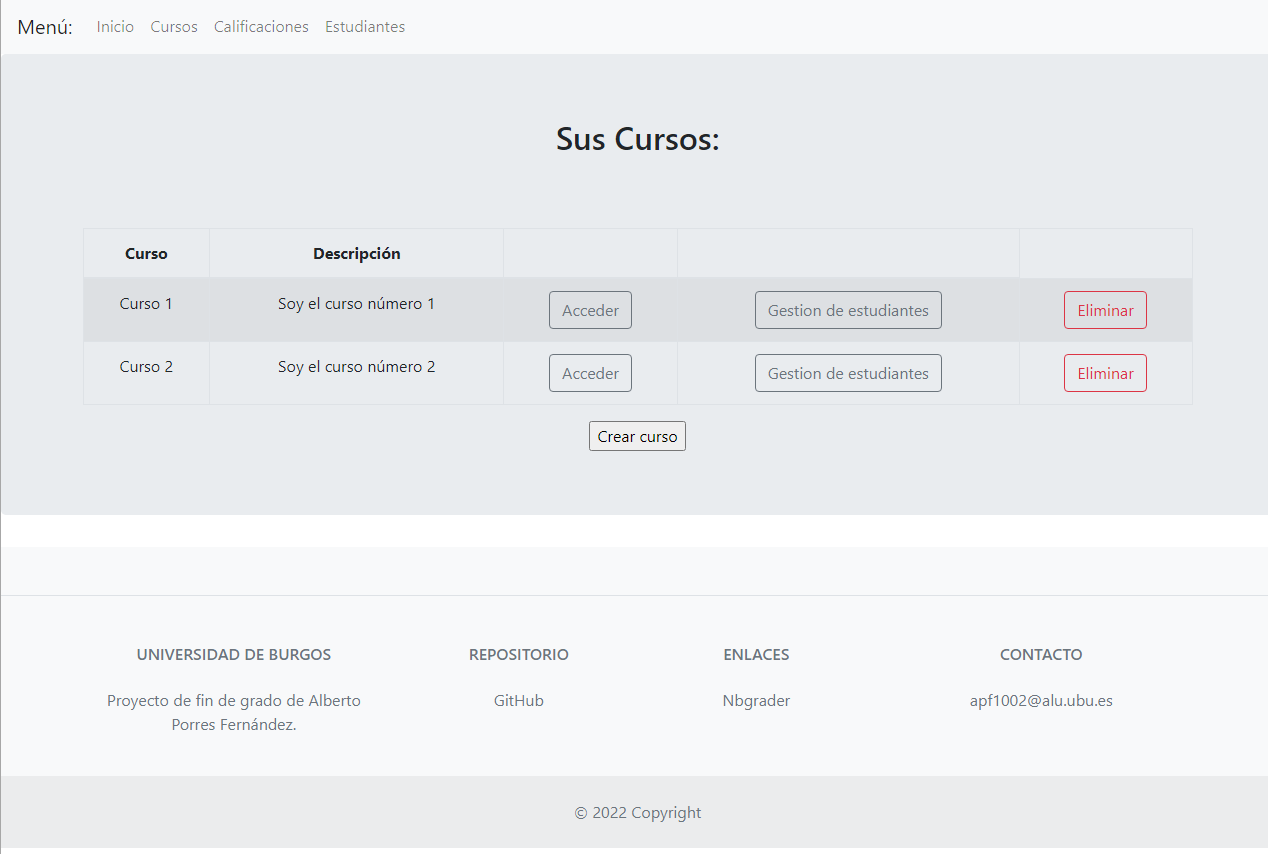
\includegraphics[width=\textwidth]{img/imgs-memoria/PaginaCursosProfesor.PNG}
\caption{Página de Cursos Profesor}
\label{PagCursosProfesor}
\end{figure}

\subsubsection{3.1 Creación de cursos}
Para la creación de un nuevo curso:
\begin{itemize}
\tightlist
\item Hacer click en el botón \textbf{Crear curso} de la \textbf{Página de Cursos del Profesor}(\ref{PagCursosProfesor}) lo cual le llevará al formulario de creación de un nuevo curso:
\begin{figure}[H]
\centering
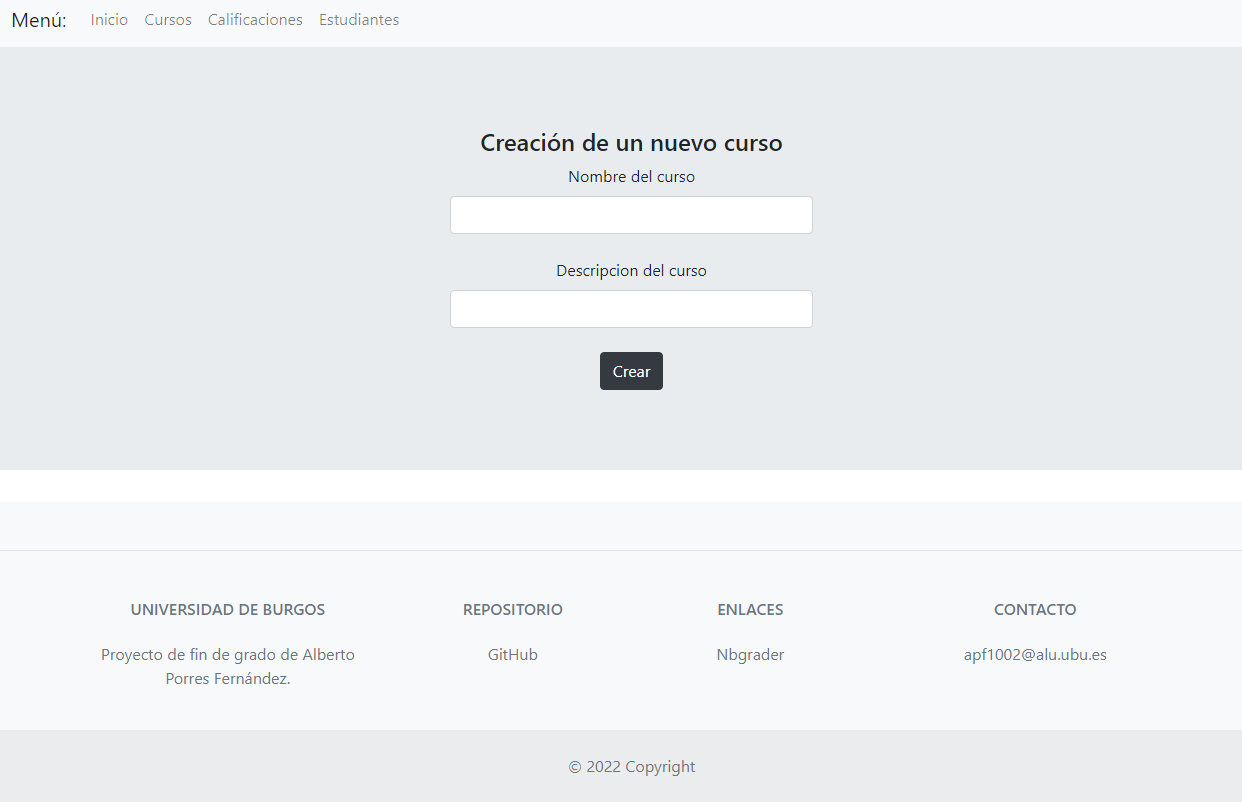
\includegraphics[width=\textwidth]{img/imgs-memoria/CrearCurso.PNG}
\caption{Página de Creación de Curso}
\end{figure}
\item Introducción de los datos (nombre y descripción) del curso a crear.
\item Hacer click en el botón \textbf{Crear}.
\item Hacer click en el botón \textbf{Confirmar} del modal de confirmación desplegado.
\item Si los datos no pertenecen a otro curso su curso será creado y visualizable desde la \ref{PagCursosProfesor} \textbf{Página de Cursos del Profesor}.
\end{itemize}


\subsubsection{3.2 Borrado de cursos}
Para el borrado de cursos se ha de hacer click en el botón \textbf{Eliminar} del curso deseado desde la \textbf{Página de Cursos}(\ref{PagCursosProfesor}), esto desplegará un modal de confirmación de acción que borrará el curso al hacer click en \textbf{Confirmar}.




\subsubsection{3.3 Gestión de alumnos de un curso}
El proceso de gestión de alumnos de un curso, que permite el ingreso o expulsión de alumnos a un curso, se realiza de la siguiente manera:
\begin{itemize}
\tightlist
\item Hacer click en el botón \textbf{Gestión de estudiantes} del curso deseado desde la \textbf{Página de Cursos}(\ref{PagCursosProfesor}). Esto nos llevará a la página de gestión de alumnos del curso:
\begin{figure}[H]
\centering
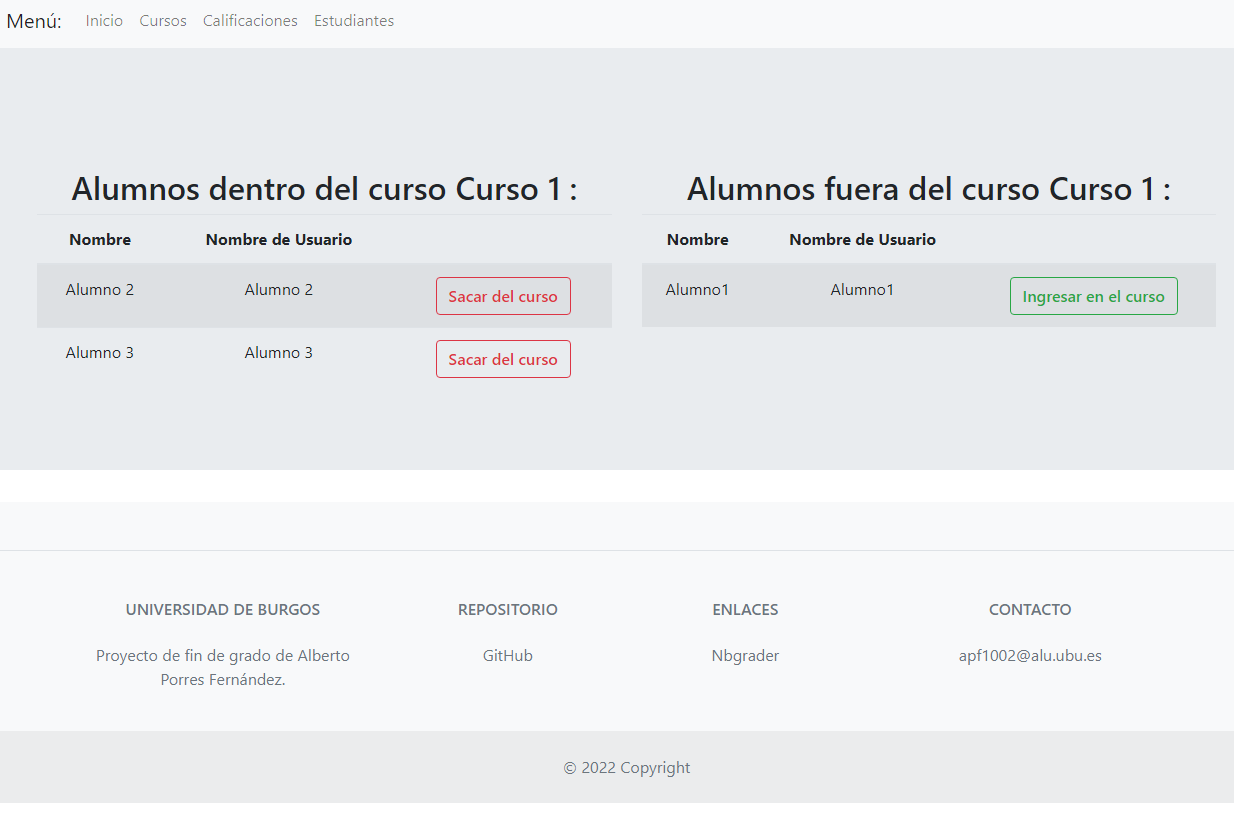
\includegraphics[width=\textwidth]{img/imgs-memoria/GestionAluCurso.PNG}
\caption{Página de Gestión de Alumnos de un Curso}
\end{figure}
\item Mediante los botones de \textbf{Sacar del curso} y \textbf{Ingresar en el curso} podrá expulsar alumnos matriculados o ingresar alumnos no matriculados al curso. La confirmación de estas acciones se hace haciendo click en el botón \textbf{Confirmar} del modal desplegado al hacer click en los botones anteriores.
\end{itemize}


\subsubsection{3.4 Acceso y gestión de contenidos de un curso}
Para ir a la página de un curso en particular, desde la que se puede realizar la gestión de su contenido, se ha de hacer click en el botón \textbf{Acceder} del curso en la \textbf{Página de Cursos del Profesor}(\ref{PagCursosProfesor}). La página/vista de un curso particular es la siguiente:
\begin{figure}[H]
\centering
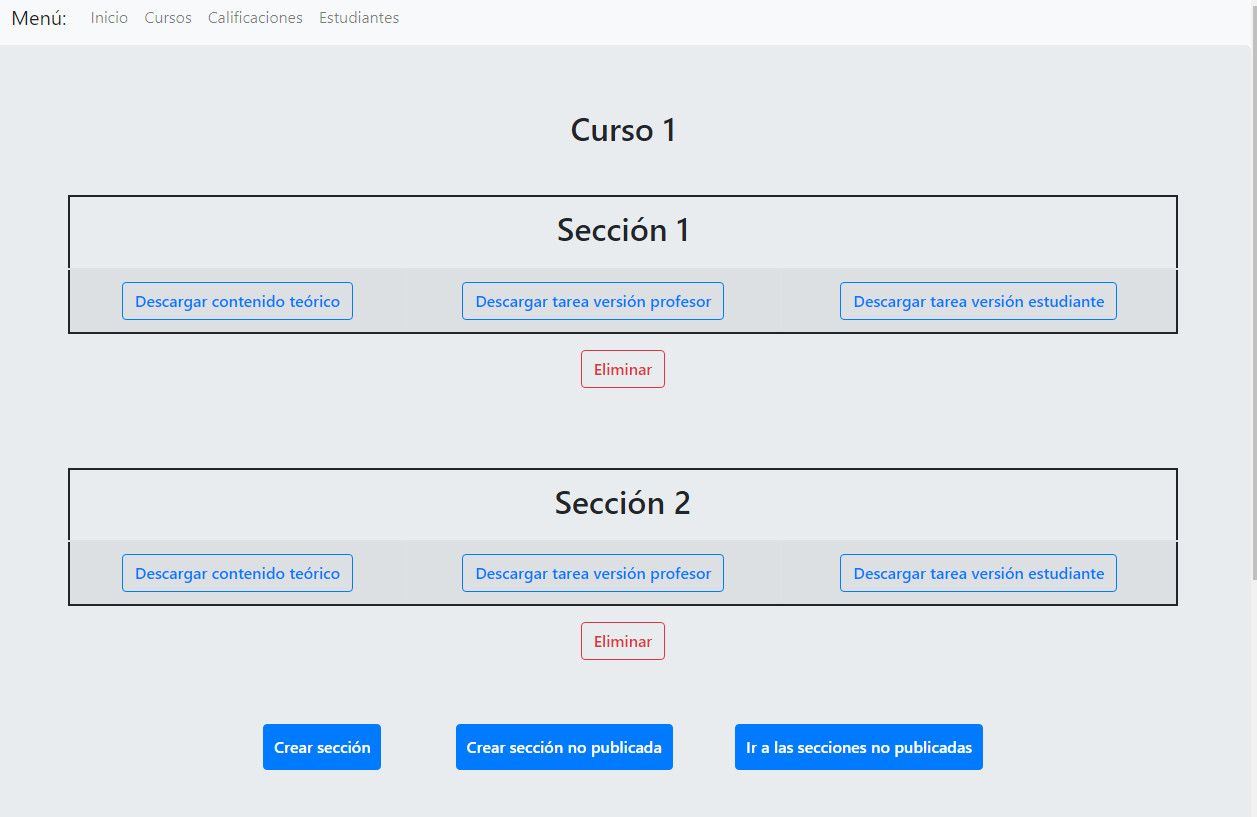
\includegraphics[width=\textwidth]{img/imgs-memoria/CursoIndividual.PNG}
\caption{Página de Gestión de Contenidos de un curso}
\label{PagContProf}
\end{figure}
Los cursos se organizan en \textbf{secciones de contenido}cada una de las cuales está \textbf{constituida por un documento teórico} cuyo formato queda a elección del profesor (PDF, DOCX, IPYNB, ...) \textbf{y una tarea corregible automáticamente en su entrega} en formato IPYNB creada mediante Jupyter Notebook y Nbgrader por el profesor. 


Desde esta vista podrá:
\begin{itemize}
\tightlist
\item Descargar contenidos teóricos, tareas en versión profesor y tareas en versión alumno a través de los botones \textbf{Descargar contenido teórico, Descargar tarea versión profesor y Descargar tarea versión alumnos} de cada sección de contenido actual del curso.
\item Eliminar secciones actuales del curso mediante el botón \textbf{Eliminar} de cada una de ellas.
\item Ir a la creación de sección de forma directa, creación de sección no publicada o gestión de las mismas (estos procesos serán descritos a continuación).
\end{itemize}

\subsubsection{3.4.1 Creación de sección de forma directa}
Para crear una sección de contenido de forma directa se ha de hacer click en el botón \textbf{Crear sección} de la \textbf{Página de gestión de contenidos de un curso}(\ref{PagContProf}) en particular, lo que nos lleva al formulario de creación de sección:

\begin{figure}[H]
\centering
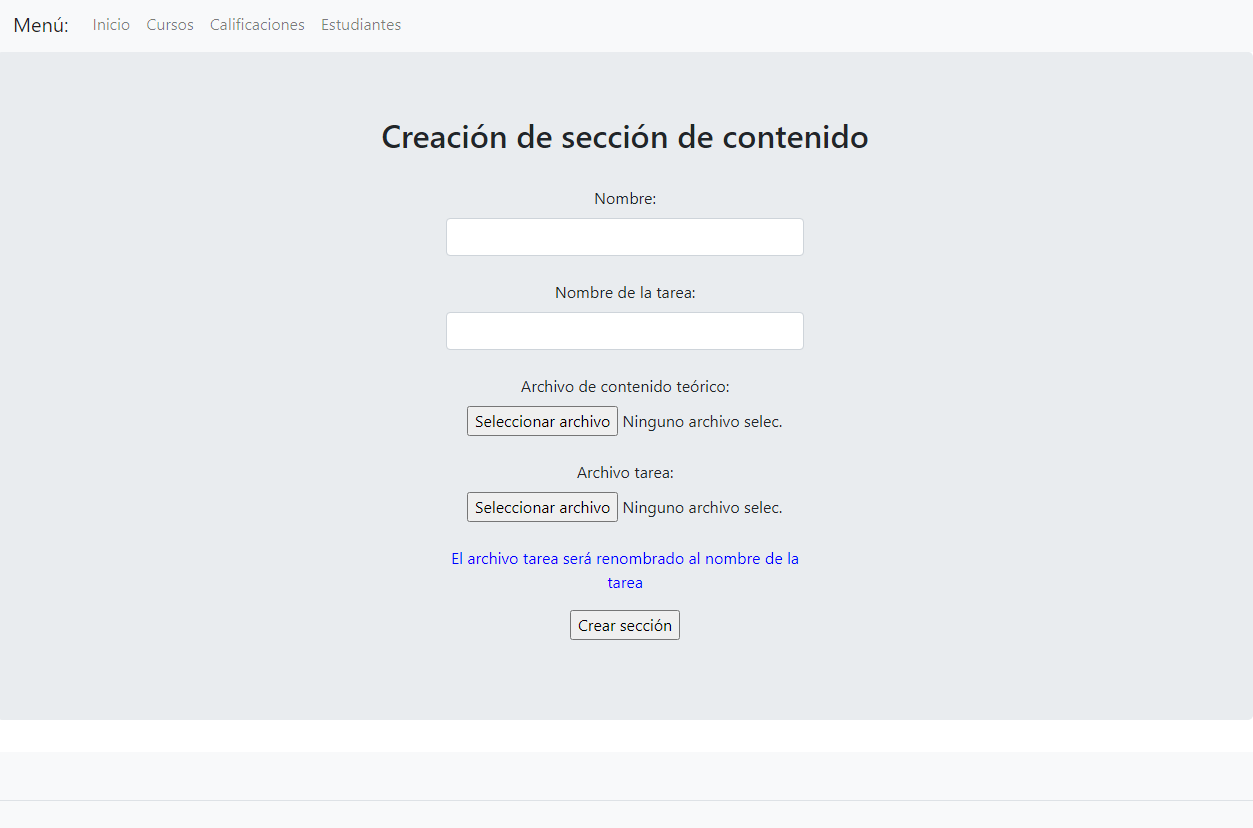
\includegraphics[width=\textwidth]{img/imgs-memoria/CrearSeccion.PNG}
\caption{Página de creación de sección}
\end{figure}

En este formulario se han de introducir el nombre de la sección, el \textbf{archivo de contenido teórico}, el \textbf{archivo tarea creado previamente mediante Jupyter Notebook y Nbgrader} y el \textbf{nombre que va a ser asignado a ese archivo tarea}. Debido al funcionamiento interno del sistema, todos los campos deben de ser únicos y no estar presentes en alguna otra sección de algún curso, de ser así la creación de la sección no será posible. 

Para crear la sección se ha de hacer click en el botón \textbf{Crear sección} que será visualizable desde la \textbf{Página de Gestión de Contenidos del Curso}(\ref{PagContProf}).

\subsubsection{3.4.2 Creación y gestión de secciones no publicadas}
Dentro de un curso también puede haber incluidas \textbf{secciones no publicadas} las cuales no son visualizables por los alumnos. La función de estas consiste en permitir a profesores la \textbf{edición de las tareas desde la propia plataforma mediante Jupyter Notebook y Nbgrader}. Haciendo click en el botón \textbf{Ir a las secciones no publicadas} de la \textbf{Página de Gestión de Contenidos del curso}(\ref{PagContProf}) irá a la página en la que se encuentran estas secciones:

\begin{figure}[H]
\centering
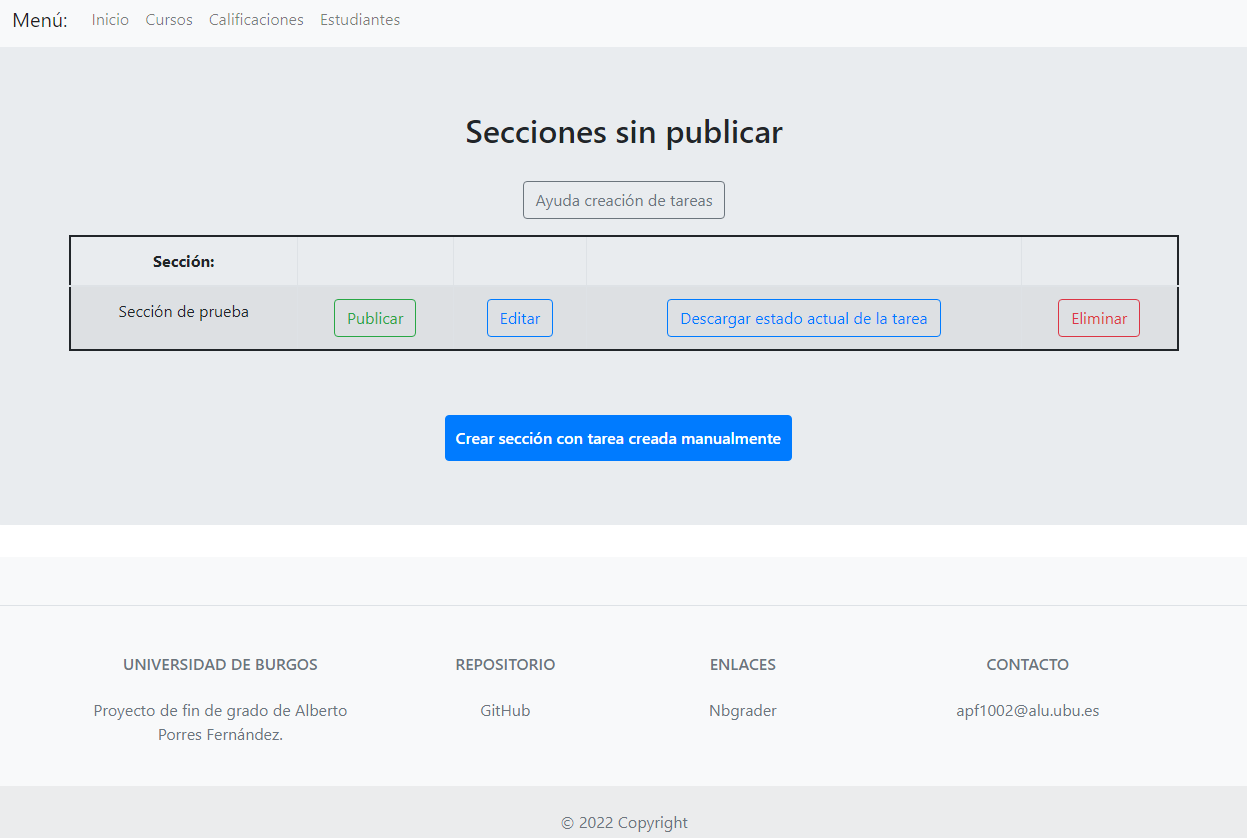
\includegraphics[width=\textwidth]{img/imgs-memoria/SeccionesNopbubli.PNG}
\caption{Página de secciones no publicadas}
\label{PagSecNoPublic}
\end{figure}

En esta vista podrá \textbf{publicar secciónes, descargar el estado actual de las tareas, eliminar secciones, crear nuevas secciones o editar las tareas desde la propia plataforma mediante el uso de los botones correspondientes visualizables en la imagen anterior}. 

Al hacer click en el botón \textbf{Editar} se le abrirá en una nueva pestaña el Notebook de Jupyter correspondiente a la tarea de la sección, permitiendo su edición. En caso de ser la primera vez que acceda desde un navegador a la edición de tareas le será \textbf{requerida una contraseña}. Esta contraseña es la palabra \textbf{''teacher''}:

\begin{figure}[H]
\centering
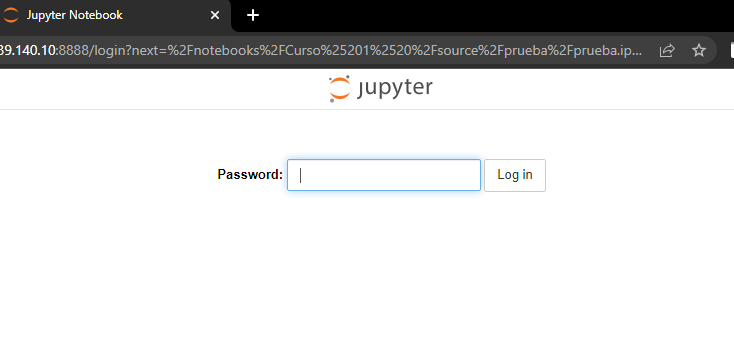
\includegraphics[width=\textwidth]{img/imgs-memoria/RequiereContra.PNG}
\caption{Requerimiento de contraseña}
\end{figure}

Una vez introducida podrá visualizar y editar la tarea correspondiente:
\begin{figure}[H]
\centering
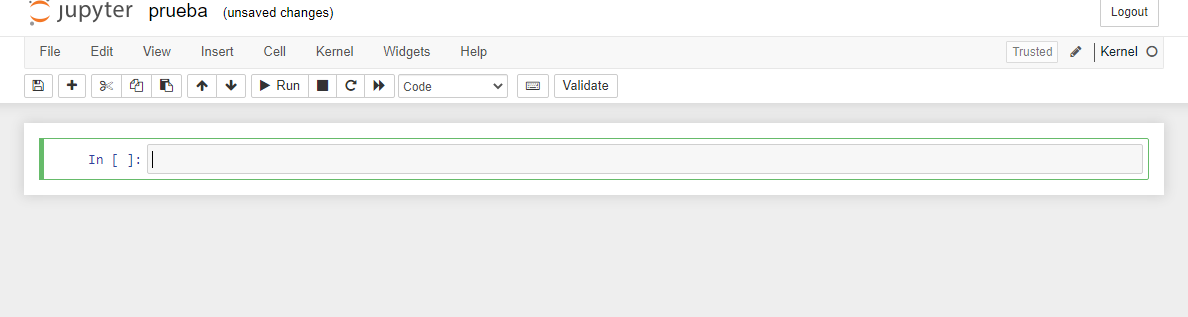
\includegraphics[width=\textwidth]{img/imgs-memoria/EdicionTareaDirecta.PNG}
\caption{Edición de tarea desde la plataforma}
\end{figure}

Para ir a la creación de secciones no publicadas se puede acceder haciendo click en el botón \textbf{Crear sección no publicada} de la \textbf{Página de Gestión de Contenidos de un curso}(\ref{PagContProf}) o haciendo click en el botón \textbf{Crear sección con tarea creada manualmente} de la \textbf{Página de secciones no publicadas}(\ref{PagSecNoPublic}). Estas acciones le llevarán al formulario de creación de secciones no publicadas:

\begin{figure}[H]
\centering
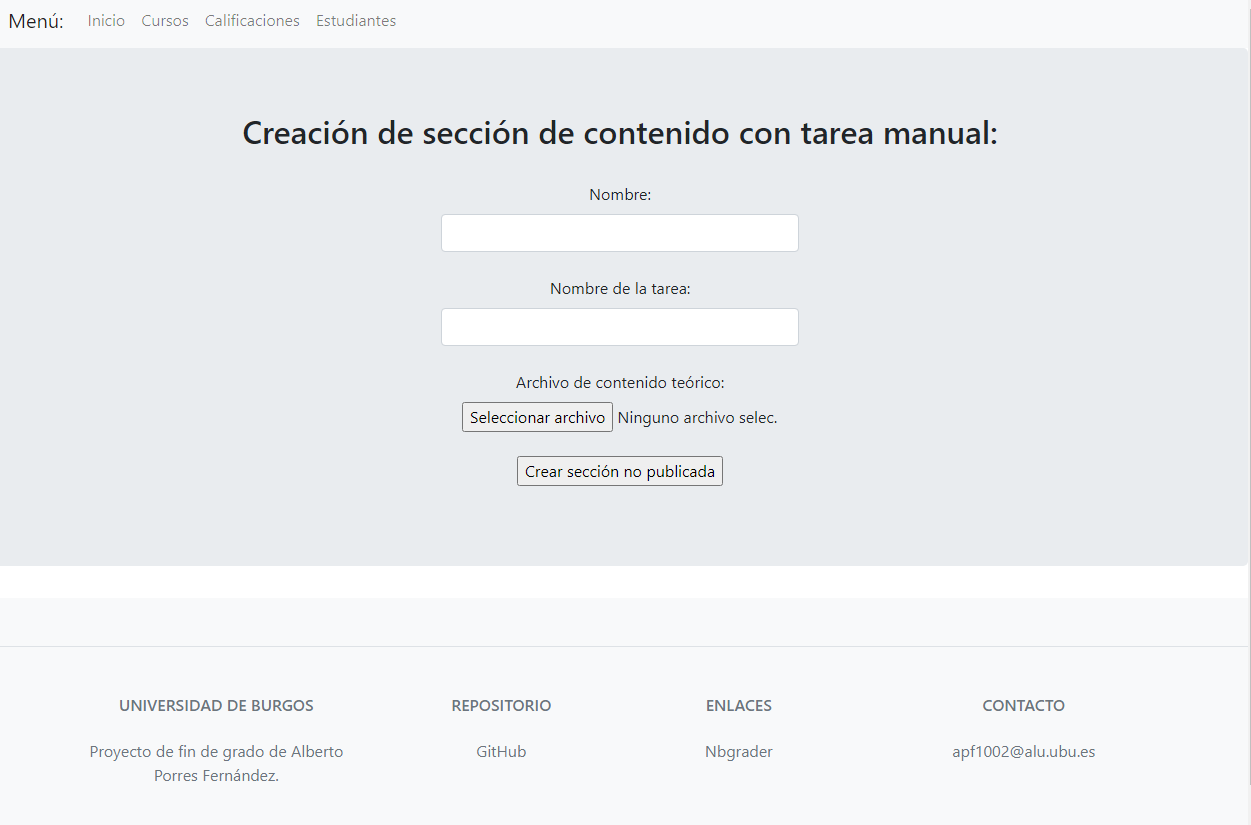
\includegraphics[width=\textwidth]{img/imgs-memoria/CrearUnreleasedSection.PNG}
\caption{Página de creación de tareas no publicadas}
\end{figure}

De la misma manera que en la creación de secciones de forma directa, todos los campos y contenidos han de ser únicos. En esta vista deberá escoger \textbf{nombre de la sección}, \textbf{nombre el cual recibirá la tarea} y entregar el \textbf{archivo de contenido teórico contendrá la sección}. La creación se realiza haciendo click en el botón \textbf{Crear sección no publicada} la cual será visualizable desde la \textbf{Página de secciones no publicadas}(\ref{PagSecNoPublic}).



\subsection{4 Crear tareas con Nbgrader}
La herramienta de la que se está haciendo uso para la creación y corrección automática de tareas dentro de la plataforma es Nbgrader. Dentro de la página de secciones no publicadas se puede acceder a la guía de esta herramienta para la creación de tareas a través del botón \textbf{Ayuda creación de tareas} pero debido a que en esta guía se cubre funcionalidades que no utilizamos, a continuación se explicará todo lo que un profesor necesita saber para la creación de tareas:

Una vez abierto el Notebook correspondiente a la tarea, ya sea desde la opción de edición proporcionada por la plataforma o de forma local teniendo instalado Jupyter Notebook y Nbgrader, se ha de activar la vista de edición de tareas en \textbf{View/Cell Toolbar/Create Assigment} en la barra navegacional del Notebook:

\begin{figure}[H]
\centering
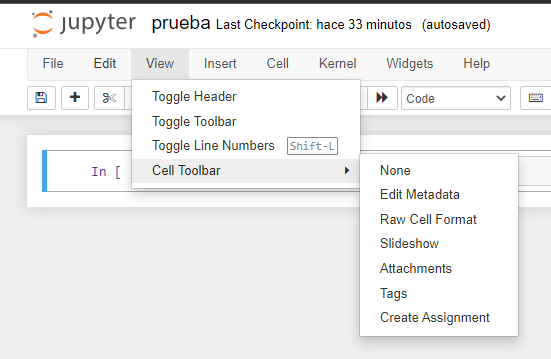
\includegraphics[width=\textwidth]{img/imgs-memoria/ActivarEdit.PNG}
\caption{Activar vista de edición}
\end{figure}

Lo que le permitirá asignar identificadores de celda a cada una de las celdas del notebook:

\begin{figure}[H]
\centering
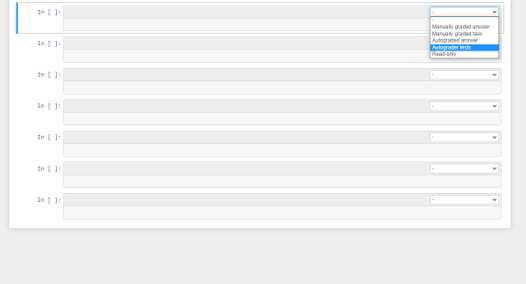
\includegraphics[width=\textwidth]{img/imgs-memoria/TipoCelda.PNG}
\caption{Tipos de celda}
\end{figure}

Los tipos de celda que nos interesan son:
\begin{itemize}
\tightlist
\item \textbf{Read-Only} Solo lectura. Estas celdas no permitirán su edición cuando sea generada la versión del alumno de la tarea.
\item \textbf{Autograded Answer} Celdas de Respuesta. En estas celdas los alumnos tendrán que implementar su código de respuesta a los ejercicios contenidos en la tarea.
\item \textbf{Autograded Test} Celdas de Test. Estas celdas contienen los test que los alumnos han de superar. A estas celdas es asignada una puntuación que los alumnos obtendrán (para ese ejercicio en particular) en caso de superar esos tests. 
\end{itemize}

Vamos a ver un ejemplo de como sería una tarea sencilla con un ejercicio a resolver y a continuación explicaremos lo que se ha hecho para comprender mejor el proceso de creación de tareas. Este ejercicio consiste en la implementación de una función que suma dos números pasados por parámetro:

\begin{figure}[H]
\centering
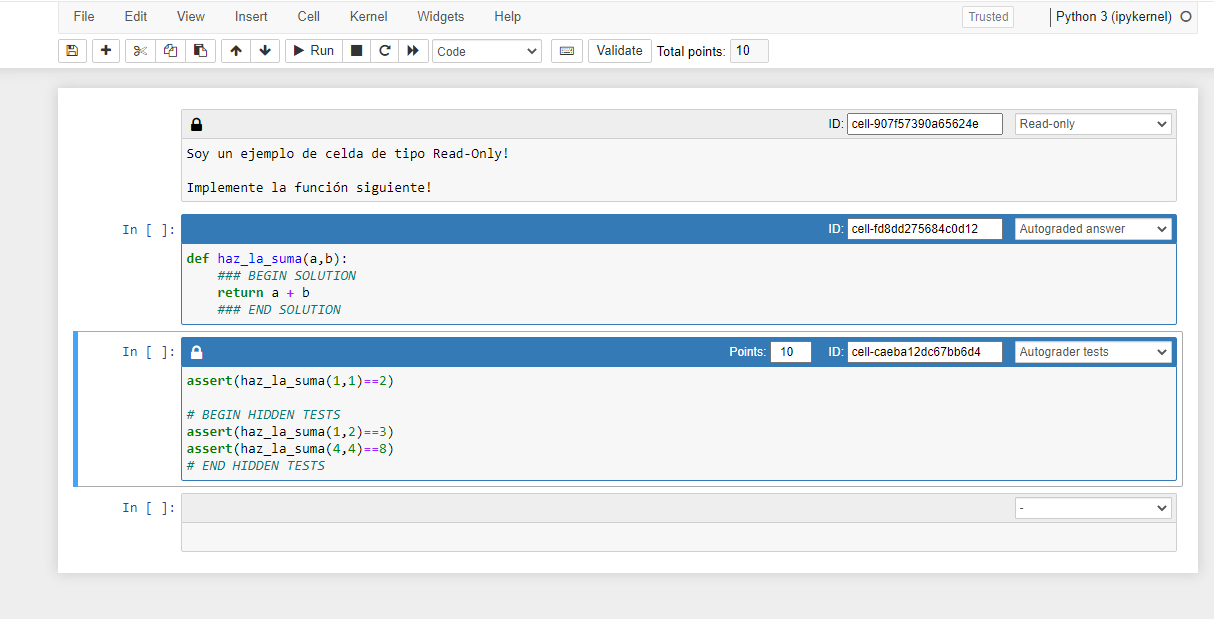
\includegraphics[width=\textwidth]{img/imgs-memoria/EjemploTarea.PNG}
\caption{Ejemplo Tarea}
\end{figure}

En la segunda celda se encuentra la función que el alumno ha de completar, Nbgrader tiene la opción de definir secciones dentro de las celdas de tipo Autograded Answer entre los comentarios \textbf{\#\#\# BEGIN SOLUTION} y \textbf{\#\#\# END SOLUTION} en las que el profesor puede implementar el código solución. Estas secciones son ocultadas en la versión de la tarea para el alumno pero son de utilidad en el desarrollo de las tareas. De forma similar, en las celdas de tipo Autograded Tests, como la tercera celda, se pueden definir secciones de test entre los comentarios \textbf{\#\#\# BEGIN HIDDEN TESTS} y \textbf{\#\#\# END HIDDEN TESTS} los cuales serán ocultados a los alumnos. Esto es de gran utilidad ya que la posibilidad de visualizar los tests pueden dar pistas sobre la resolución de los problemas a los alumnos. Se tendrá cuidado al definir estos tipos de secciones ya que un fallo en la ortografía de los comentarios provocará que la tarea \textbf{no se genere}. 

Como podemos ver en la imagen superior, a la tercera celda le ha sido asignada una puntuación como se ha descrito anteriormente.  Nbgrader no redondea la puntuación total de todos los ejercicios de una tarea, sin embargo, se ha adaptado la plataforma para que la calificación obtenida cuando un alumno envía una tarea sea \textbf{sobre 10} pese a que la suma total de puntuaciones de una tarea pueda ser diferente.

Adicionalmente y como podemos ver en la barra navegacional del Notebook, Nbgrader añade un botón \textbf{Validate} que permite a los profesores comprobar si el código que ha implementado dentro de los comentarios de solución pasan los tests.

\begin{figure}[H]
\centering
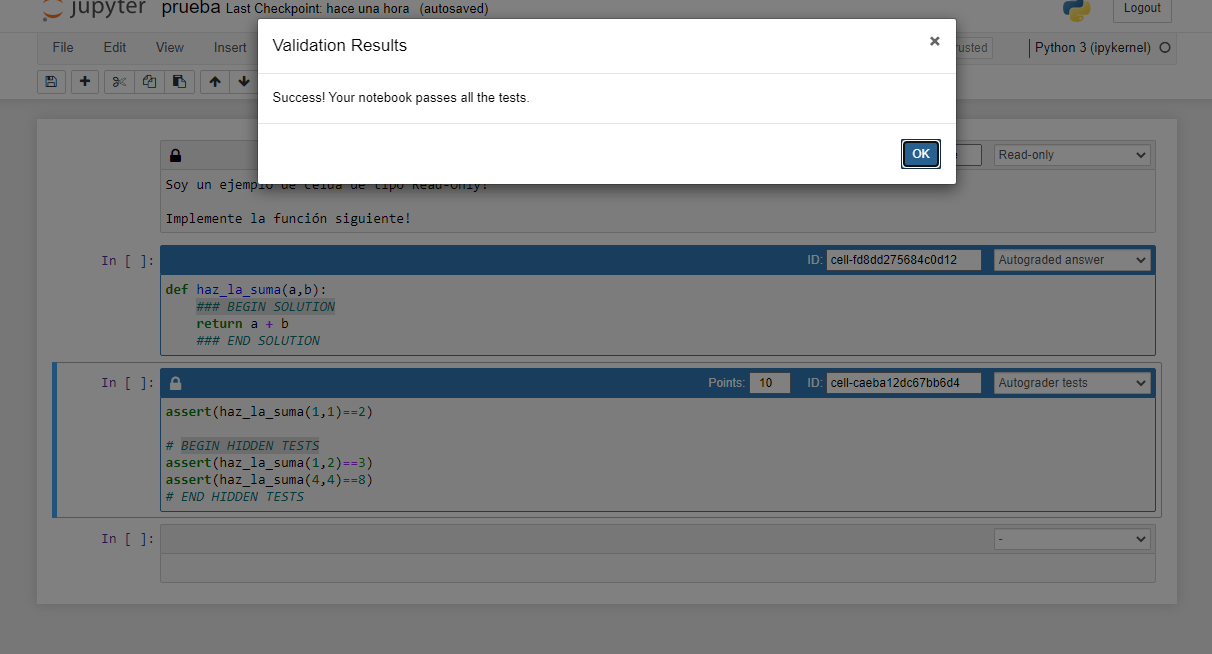
\includegraphics[width=\textwidth]{img/imgs-memoria/Succes!.PNG}
\caption{Ejemplo validate}
\end{figure}

La forma en la que Nbgrader comprueba la superación de los ejercicios al ser ejecutada la orden de corrección es mediante la detección de errores. Cuando una celda es de tipo \textbf{Autograded Test} y la ejecución de estos ha resultado en algún error, la puntuación obtenida en ese ejercicio es 0 o la asignada a la celda en caso contrario. Por ello, queda a decisión de los profesores la forma en la que implementan sus tests. En el ejemplo anterio se está haciendo uso del método \textbf{assert} de Python.

La versión de los estudiantes de la tarea anterior, tras ser generada al crear una sección de forma directa o al ser publicada una sección no publicada, es la siguiente:


\begin{figure}[H]
\centering
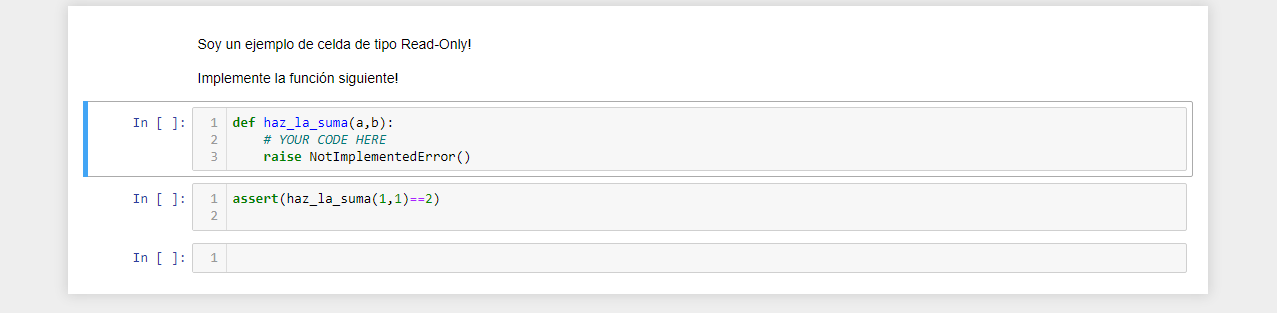
\includegraphics[width=\textwidth]{img/imgs-memoria/VAlumno.PNG}
\caption{Ejemplo versión alumno}
\end{figure}

Como podemos ver, el código implementado por el profesor y los tests ocultos no son visualizables.



\subsection{5 Acceso a todas las calificaciones}
Para poder acceder a la página calificaciones global de todos los alumnos en sus cursos se ha de hacer click en el botón \textbf{Ir a las calificaciones} de la \ref{PagProfesor} \textbf{Página principal del profesor} o en el botón \textbf{Calificaciones} de la barra navegacional superior. Esta página es la siguiente:

\begin{figure}[H]
\centering
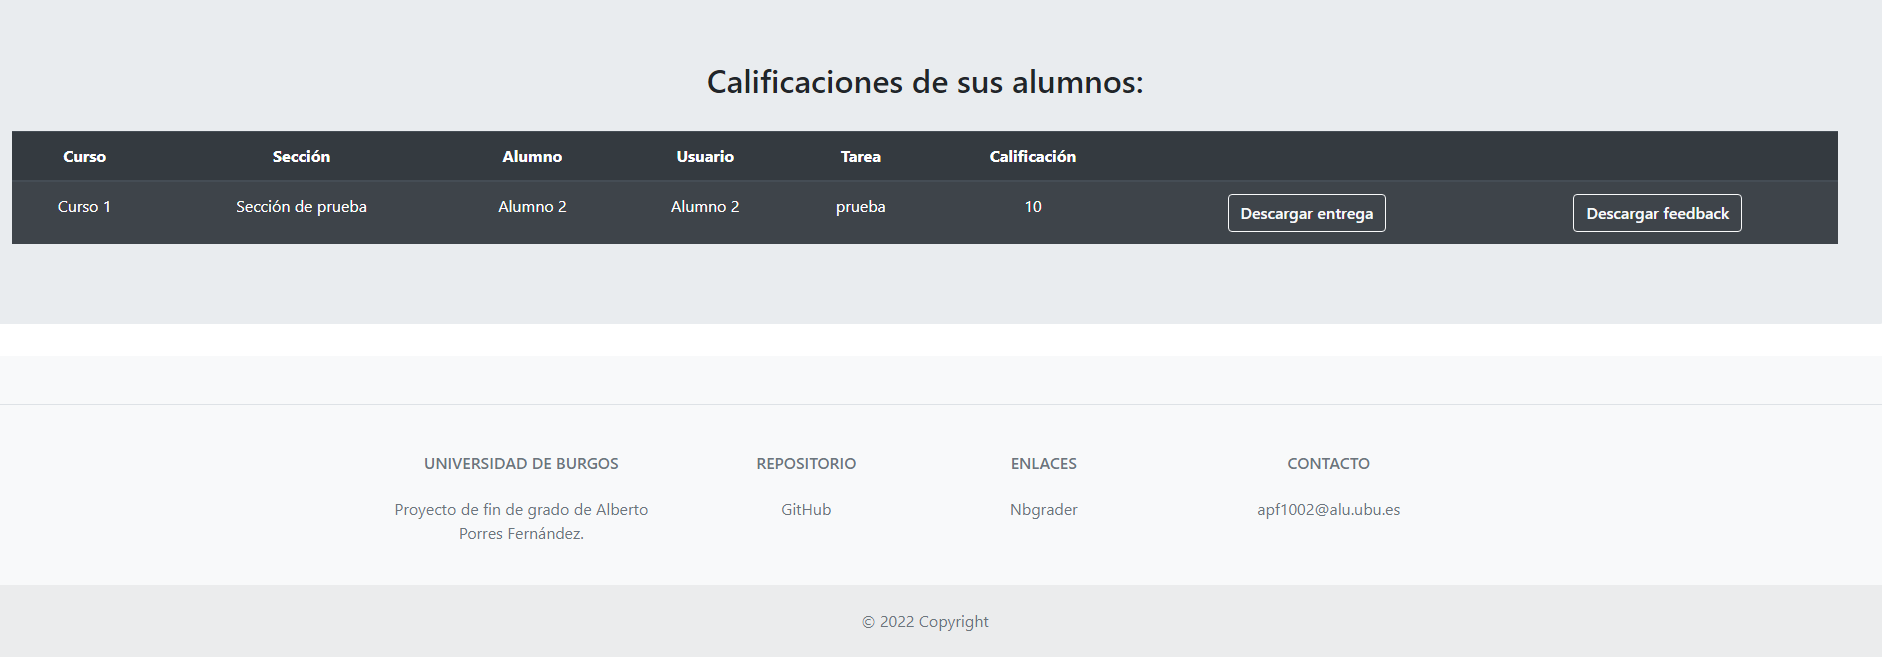
\includegraphics[width=\textwidth]{img/imgs-memoria/califGlobal.PNG}
\caption{Página de calificaciones global}
\end{figure}

En ella tendrá acceso a la descarga del archivo tarea entregado por el alumno mediante el botón \textbf{Descargar entrega} y a la descarga del documento feedback generado tras la calificación automática medainte el botón \textbf{Descargar Feedback}


\subsection{6 Gestión de alumnos}
Para poder acceder a la página gestión de alumnos click en el botón \textbf{Ir a la gestión de alumnos} de la \textbf{Página principal del profesor}(\ref{PagProfesor}) o en el botón \textbf{Estudiantes} de la barra navegacional superior. Esta página es la siguiente:

\begin{figure}[H]
\centering
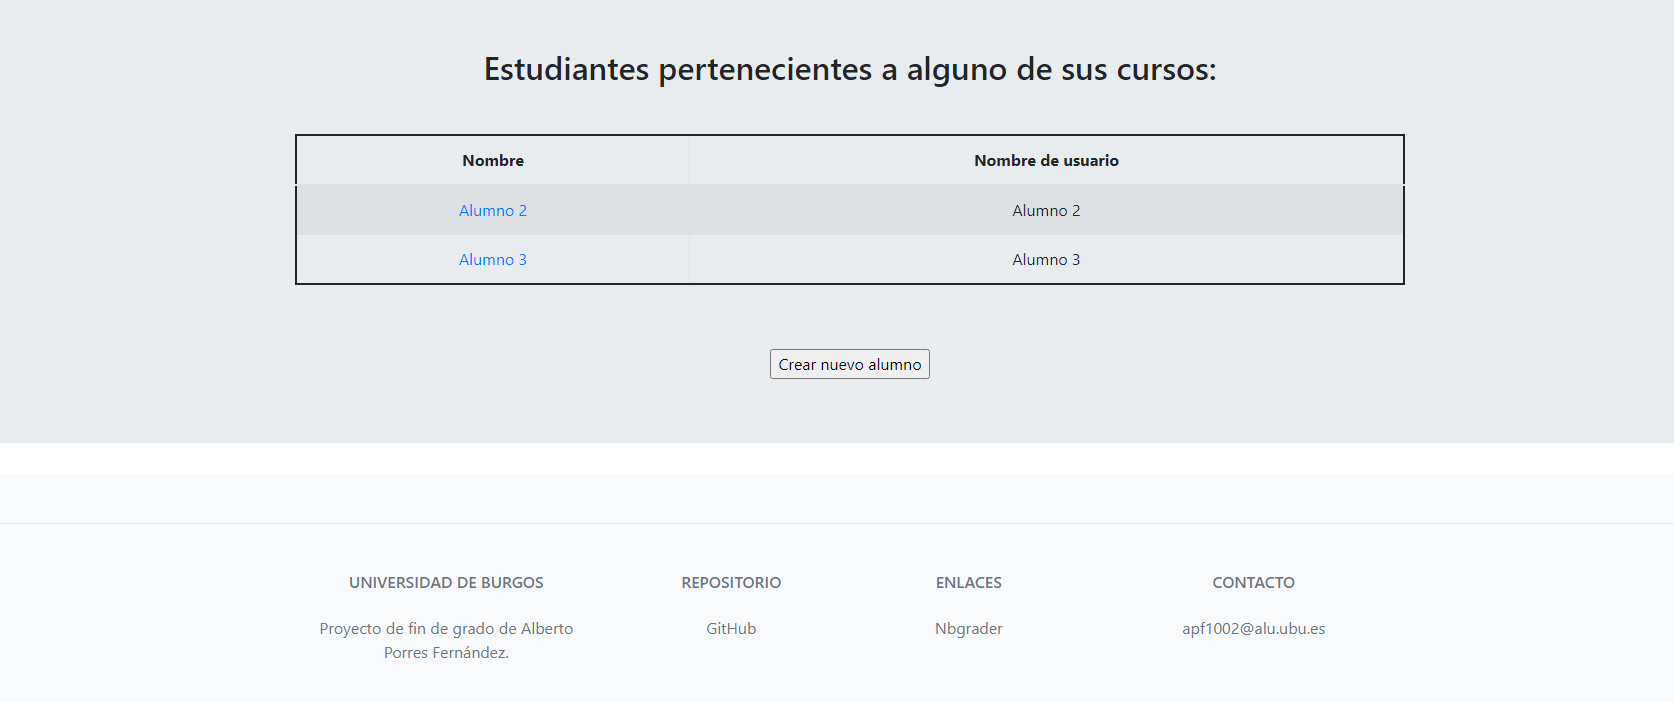
\includegraphics[width=\textwidth]{img/imgs-memoria/paginaEstudiantes.PNG}
\caption{Página de gestión alumnos}
\end{figure}


\subsubsection{6.1 Creación de alumnos}
Al hacer click en el botón \textbf{Crear nuevo alumno} de la página de estudiantes irá al formulario de creación de alumno:

\begin{figure}[H]
\centering
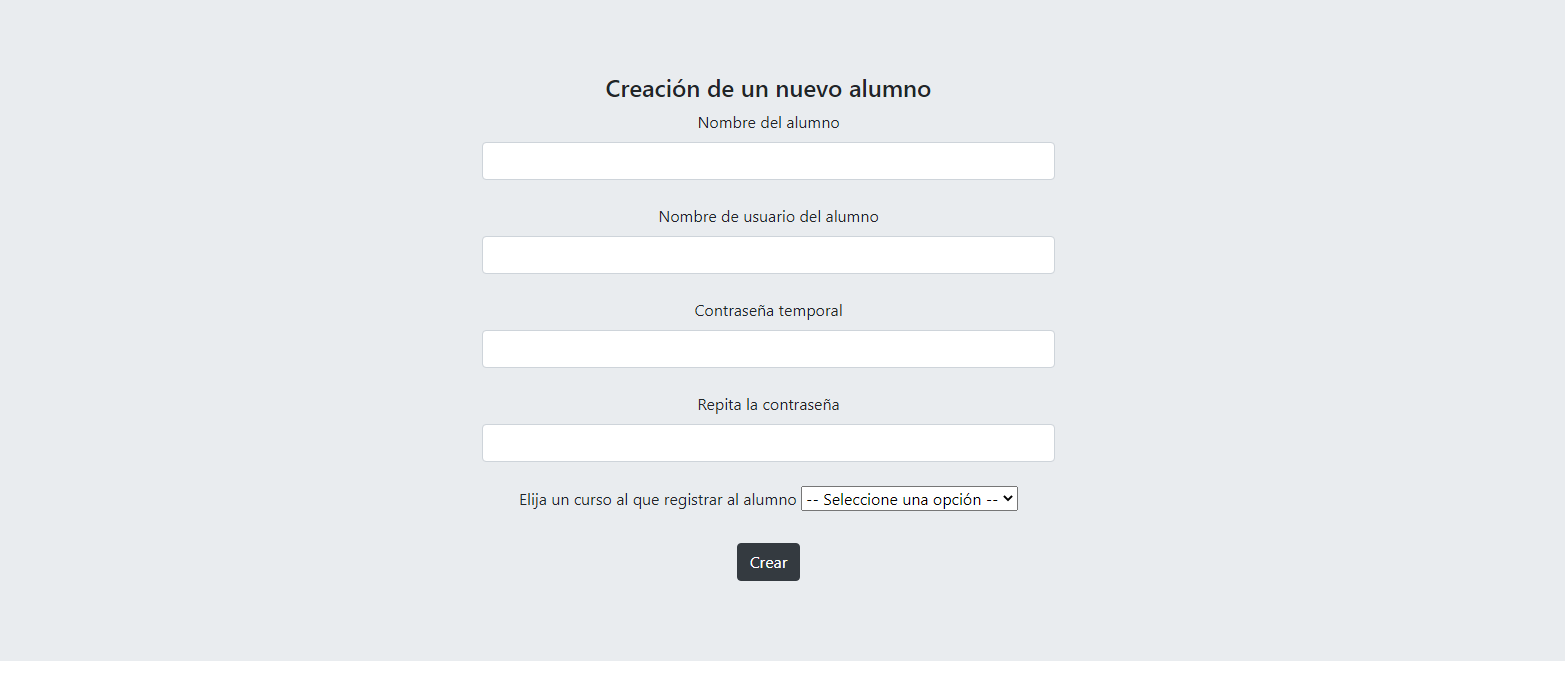
\includegraphics[width=\textwidth]{img/imgs-memoria/crearAlumno.PNG}
\caption{Página de creación de alumno}
\label{PagGesAlu}
\end{figure}

En ella deberá introducir su \textbf{nombre, el nombre de usuario de su cuenta, la contraseña temporal de esta y el curso al que quiere registrar al nuevo alumno}.

Si el nombre de usuario escogido para el alumno no pertenece a otro alumno este será creado de forma correcta y visualizable desde la \textbf{Página de gestión alumnos}(\ref{PagGesAlu}).

\subsubsection{6.2 Perfil del alumno}
Al hacer click en el nombre un alumno en la \textbf{Página de gestión alumnos}(\ref{PagGesAlu}) irá al perfil de calificaciones del alumno:

\begin{figure}[H]
\centering
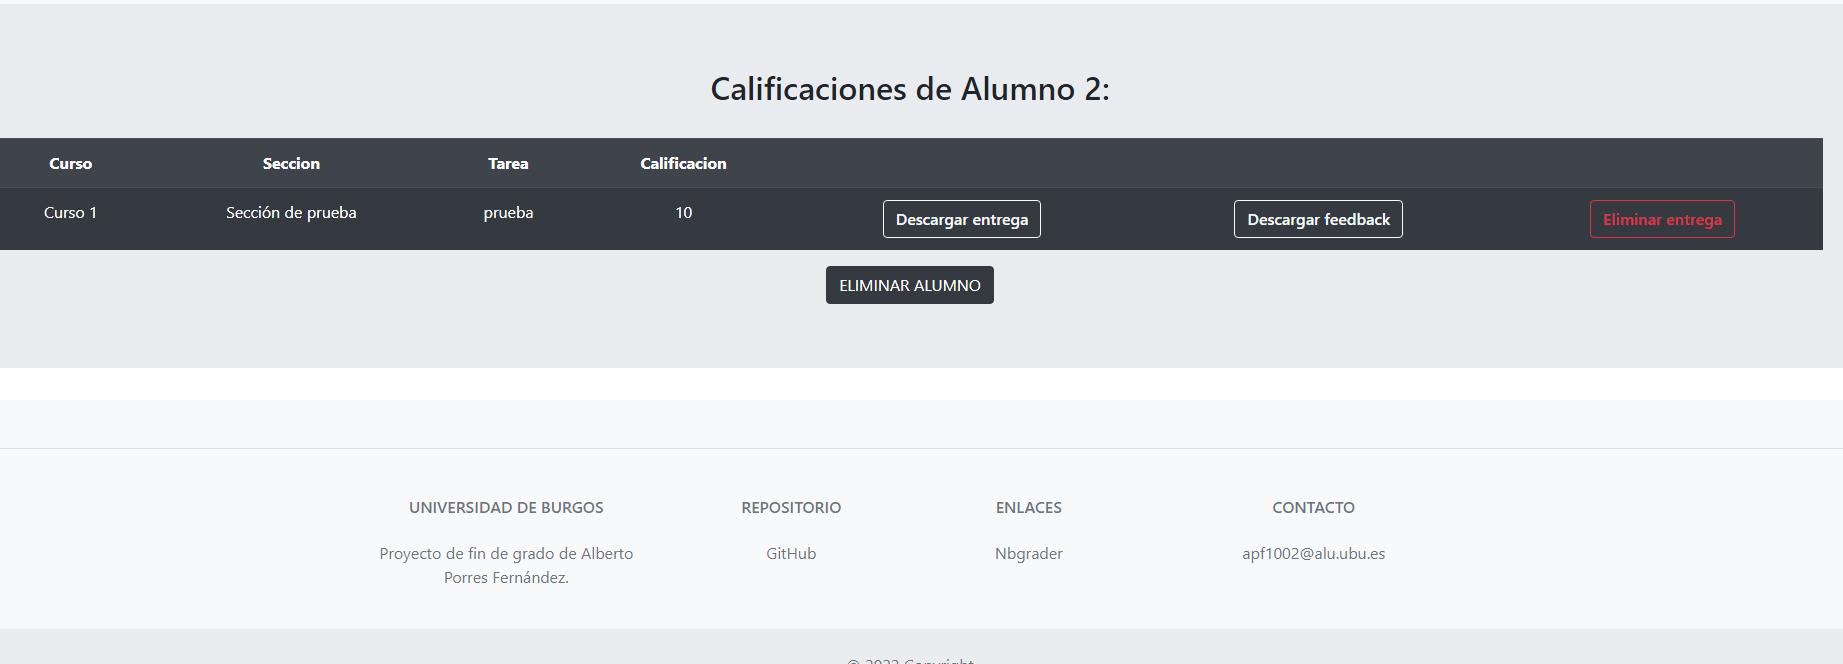
\includegraphics[width=\textwidth]{img/imgs-memoria/califAlumno.PNG}
\caption{Página de perfil del alumno}
\end{figure}

Desde esta podrá consultar las calificaciones de este, descargar los documentos de entrega y feedback como en la página de calificaciones globar y adicionalmente:

\begin{itemize}
\tightlist
\item \textbf{Eliminar entregas del estudiante} Al hacer click en el botón \textbf{Eliminar entrega} de la calificación, lo que permitirá al alumno volver a entregar la tarea de nuevo.
\item \textbf{Eliminar la cuenta del alumno} Al hacer click en el botón \textbf{ELIMINAR ALUMNO}. Se ha de tener en cuenta al realizar esta acción que un alumno puede estar inscrito a cursos de otros profesores.
\end{itemize}


\subsection{7 Cambio de contraseña}
Para acceder al cambio de contraseña de su cuenta se ha de hacer click en el botón \textbf{Cambiar Contraseña} de la \textbf{Página principal del profesor}(\ref{PagProfesor}). Esto le llevará al formulario de cambio de contraseña:

\begin{figure}[H]
\centering
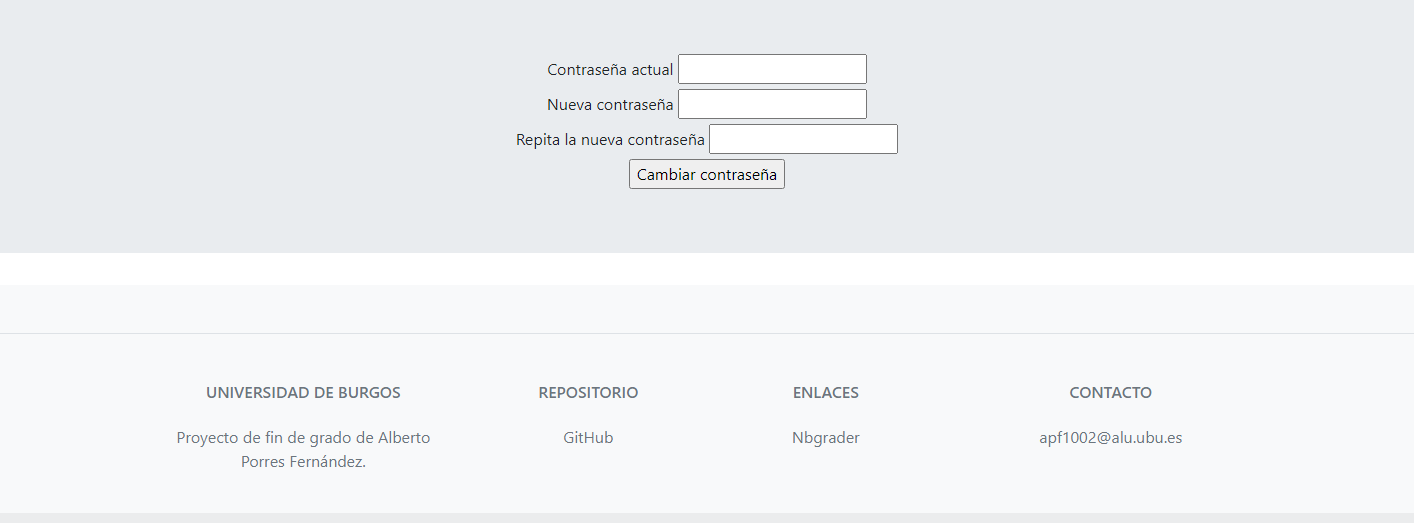
\includegraphics[width=\textwidth]{img/imgs-memoria/CambiarContra.PNG}
\caption{Página de cambio de contraseña del profesor}
\end{figure}

Al completar el formulario y aceptar el modal de confirmación emergente, su sesión será cerrada siendo redireccionado al login.

\subsection{8 Cierre de sesión} 
El cierre de sesión se realiza haciendo click en el botón \textbf{Cerrar Sesión} de la \textbf{Página principal del profesor}(\ref{PagProfesor}) y aceptando el modal de confirmación emergente.



\newpage

\section{Manual del alumno}
A continuación se explicará el manejo de la plataforma orientado a los alumnos:

\subsection{1 Acceso a la plataforma}
El acceso a la plataforma es realizado a través del siguiente enlace: \url{http://3.89.140.10/} el cual nos lleva a la página inicial de esta.

\begin{figure}[H]
    \centering
    
\includegraphics[width=\textwidth]{img/imgs-memoria/Landing.PNG}
    \caption{Página inicial}
\end{figure}

\subsection{2 Inicio de Sesión}
El proceso de inicio de sesión contiene los siguientes paso:
\begin{itemize}
\tightlist
    \item Una vez accedido a la Página incial hacer click en el botón \textbf{Acceder} lo cual nos llevará a la página de inicio de sesión:
        \begin{figure}[H]
        \centering
        
\includegraphics[width=\textwidth]{img/imgs-memoria/InicioSesion.PNG}
        \caption{Pagina Inicio de sesión}
        \end{figure}
    \item Introducir los credenciales de inicio de sesión y hacer click en el botón \textbf{Login}.
    \item Si los credenciales son correctos será llevado a la \textbf{Página principal del alumno}:
        \begin{figure}[H]
        \centering
        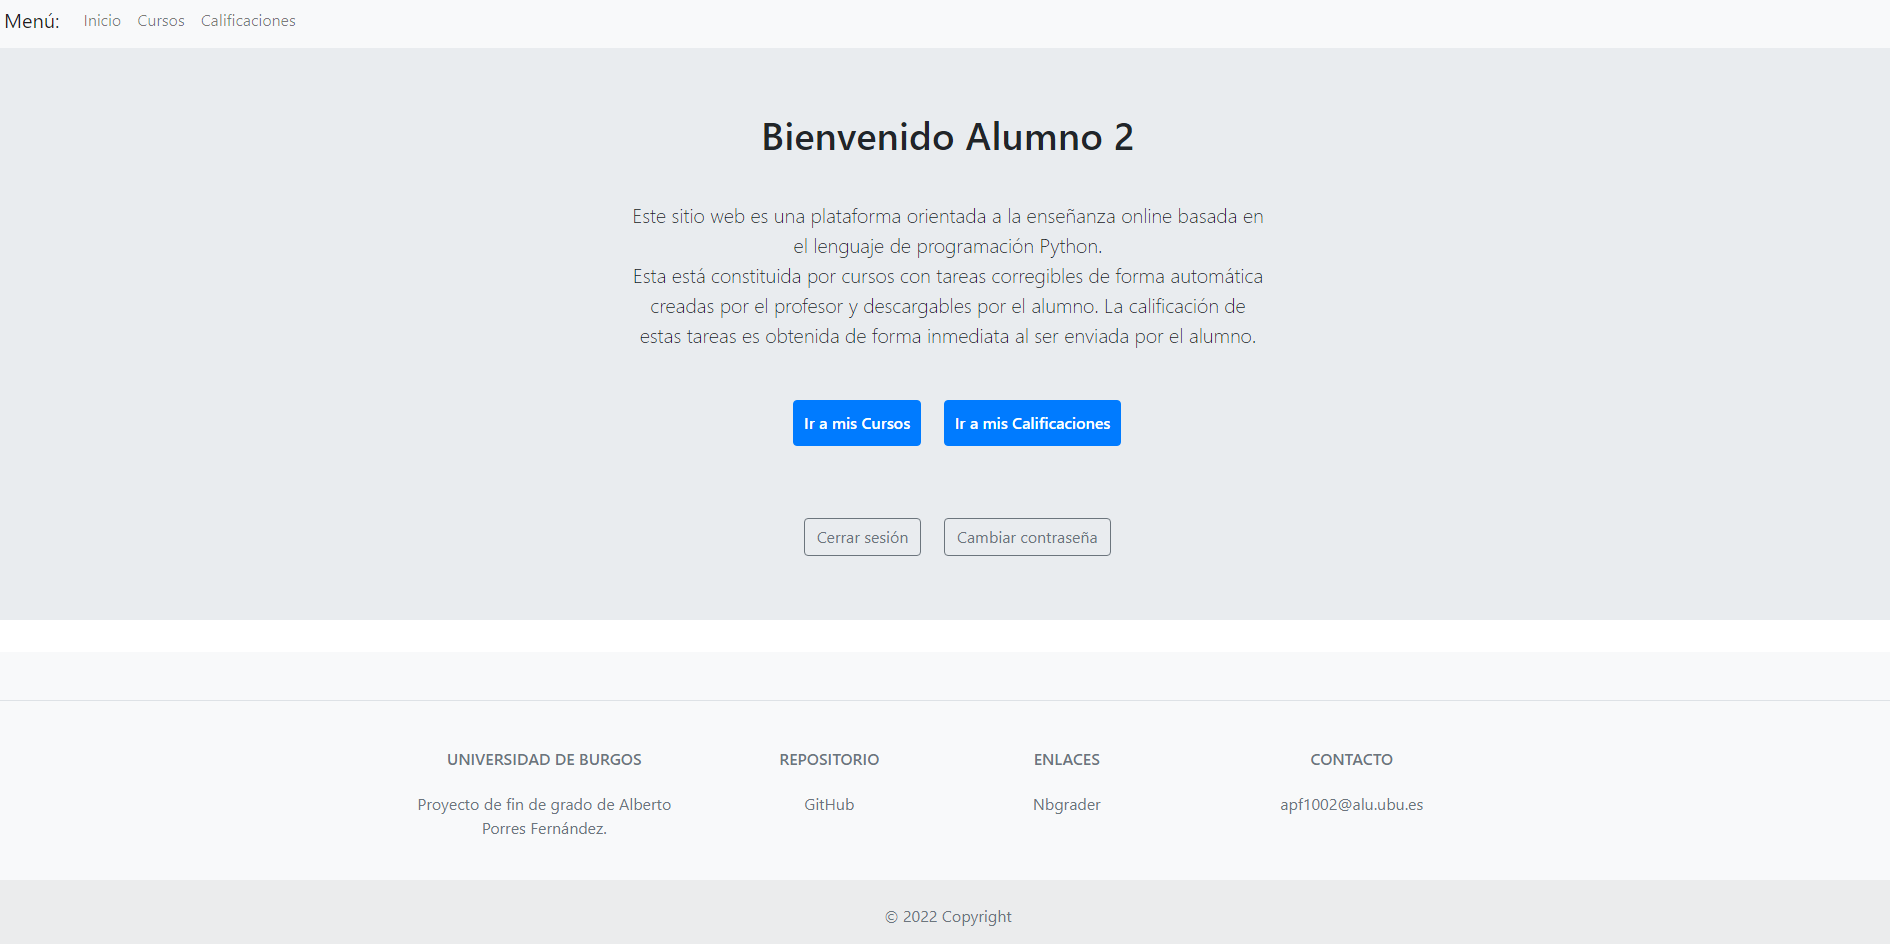
\includegraphics[width=\textwidth]{img/imgs-memoria/StudentMain.PNG}
        \caption{Página Principal Alumno}
        \label{PagAlumno}
        \end{figure}
    \item En caso de ser su \textbf{primer inicio de sesión en la plataforma deberá realizar el cambio de contraseña} por lo que será redireccionado directamente a esta página.
\end{itemize}

\subsection{3 Acceso a Cursos}
Para acceder a los cursos a los que el alumno está inscrito ha de hacer click en el botón \textbf{Ir a mis cursos} de la \textbf{Página principal del alumno}(\ref{PagAlumno}) o en el botón \textbf{Cursos} de la barra navegacional superior. Esto le llevará a la \textbf{Página de cursos del alumno}:
\begin{figure}[H]
\centering
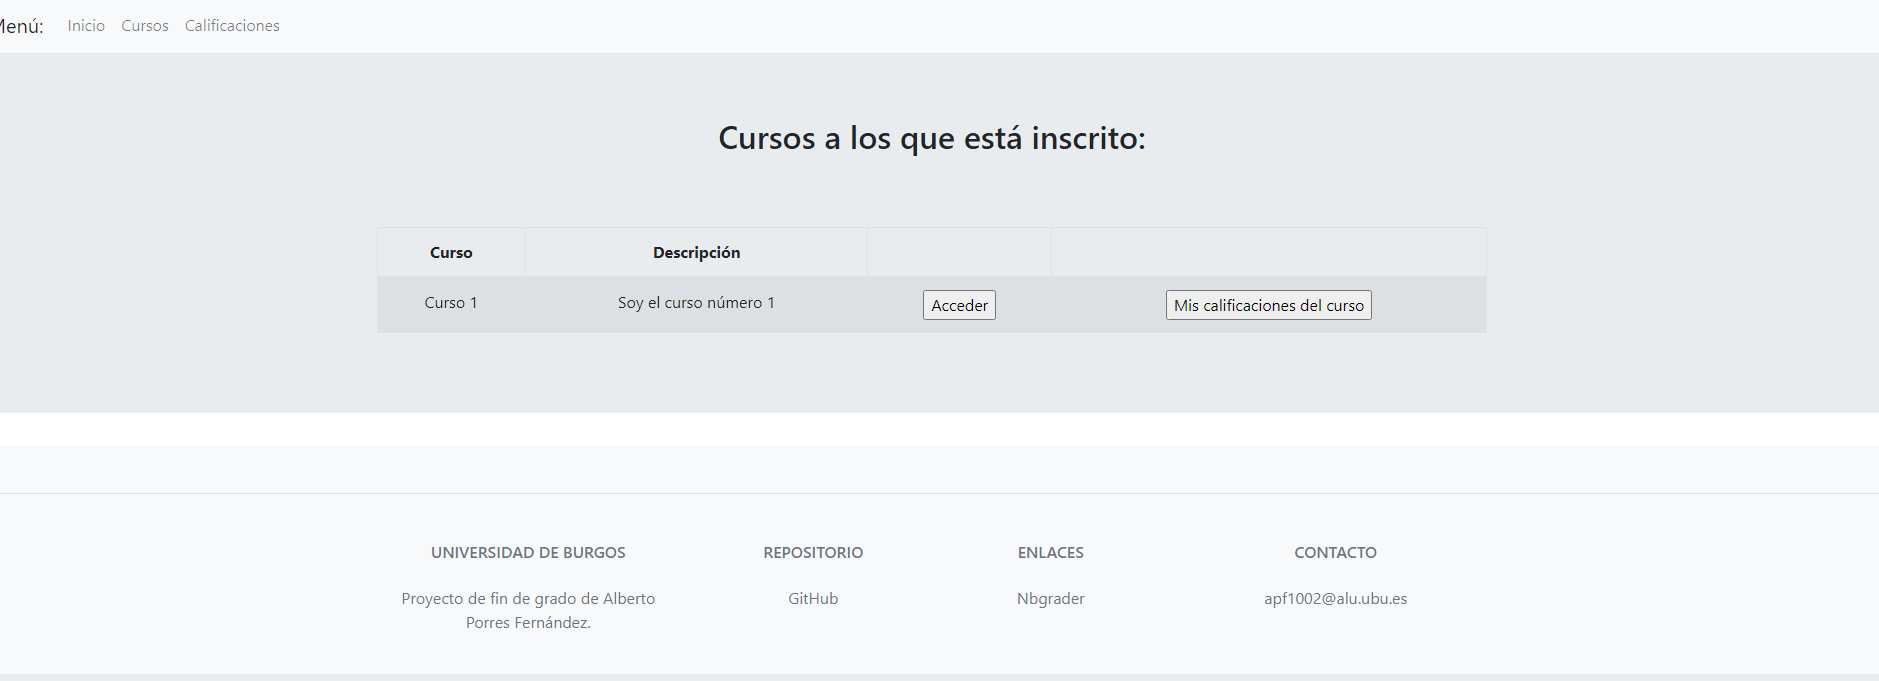
\includegraphics[width=\textwidth]{img/imgs-memoria/CursosAlumno.PNG}
\caption{Página de Cursos del alumno}
\label{PagCurAlu}
\end{figure}

\subsubsection{3.1 Acceso a contenidos del curso}
Una vez en la \textbf{Página de cursos del alumno} a los que este está inscrito, para acceder al contenido del curso ha de hacer click en el botón \textbf{Acceder} del curso deseado. Esto le llevará a la \textbf{Página de contenidos del curso}:

\begin{figure}[H]
\centering
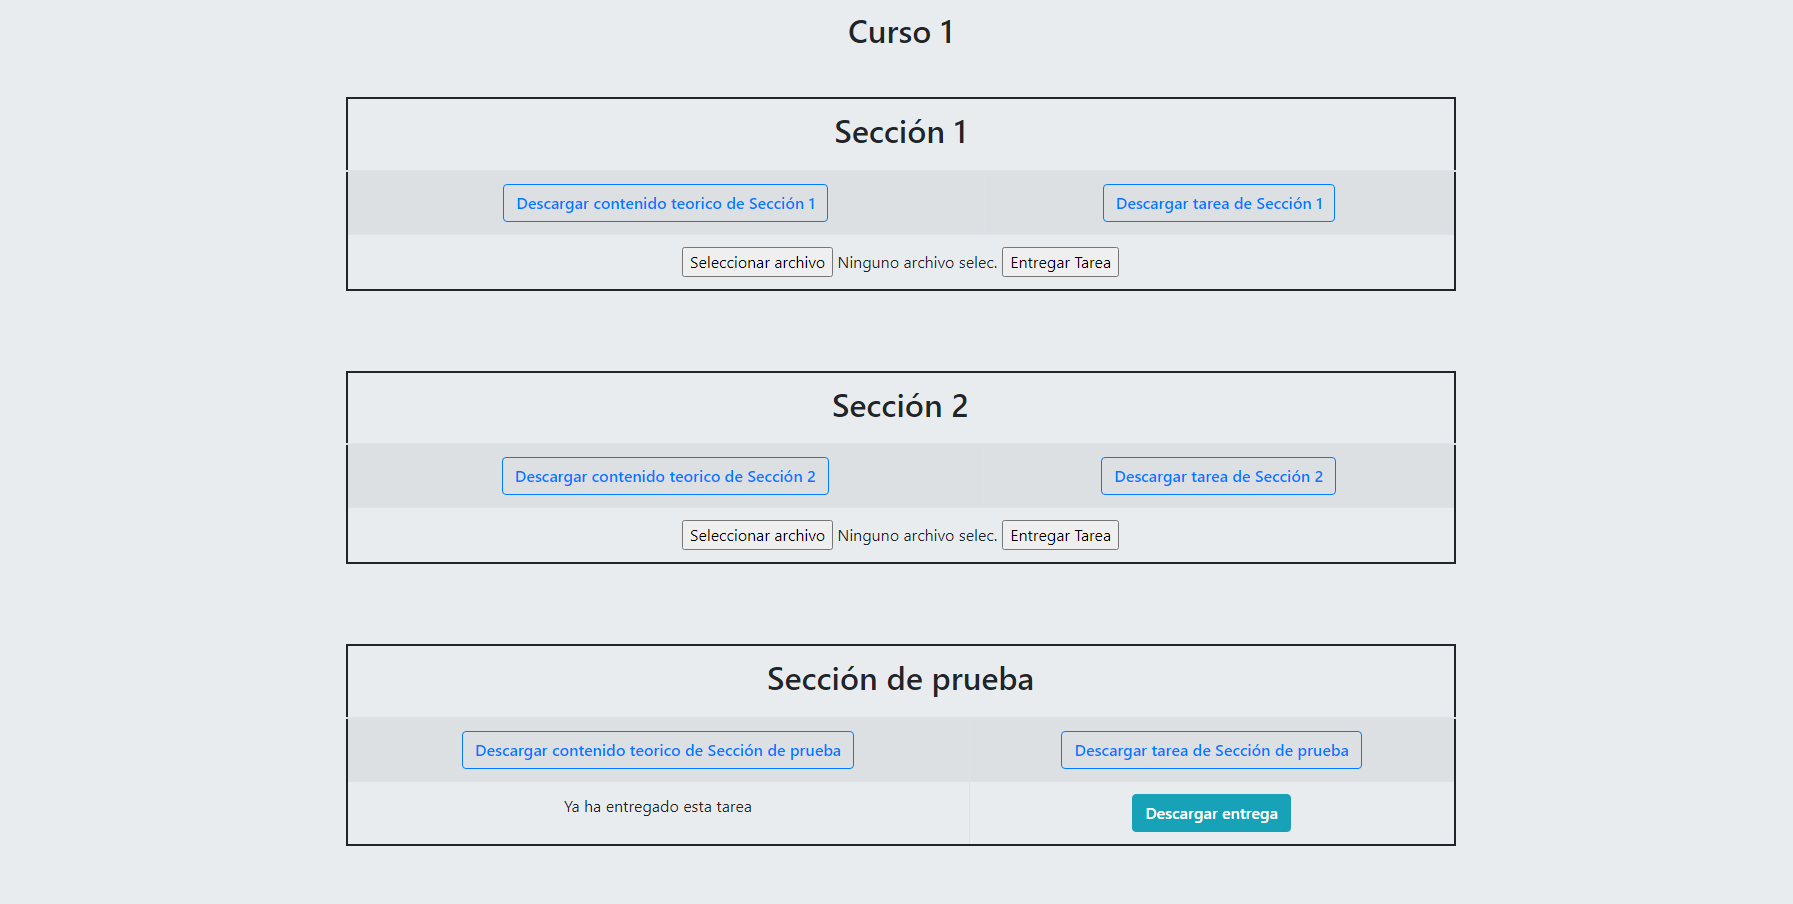
\includegraphics[width=\textwidth]{img/imgs-memoria/ContenidoCurso.PNG}
\caption{Página de Contenidos del Curso}
\label{PagContentAlu}
\end{figure}

Los cursos están consituidos por secciones de contenido cada una de las cuales contiene un documento teórico y una tarea a entregar como se puede ver en la imagen anterior. En esta página podrá:
\begin{itemize}
\tightlist
\item Descargar los contenidos teóricos y tareas de cada sección mediante los botones \textbf{Descargar contenido teórico} y \textbf{Descargar tarea} de cada una.
\item Realizar la entrega de tareas mediante el formulario de entrega de cada sección.
\item Descargar los documentos tarea previamente entregados en aquellas secciones en las que la tarea ya se encuentre enviada mediante el botón \textbf{Descargar entrega} de la sección. En el caso de que un profesor elimine una entrega tendrá habilitada de nuevo el envío de la tarea para la sección.
\end{itemize}


\subsubsection{3.2 Acceso a calificaciones del curso}
Para consultar las calificaciones obtenidas en un curso específico ha de hacer click en el botón \textbf{Mis calificaciones del curso} en la \textbf{Página de cursos del alumno}(\ref{PagCurAlu}).Esto le llevará a la \textbf{Página de calificaciones del curso}:

\begin{figure}[H]
\centering
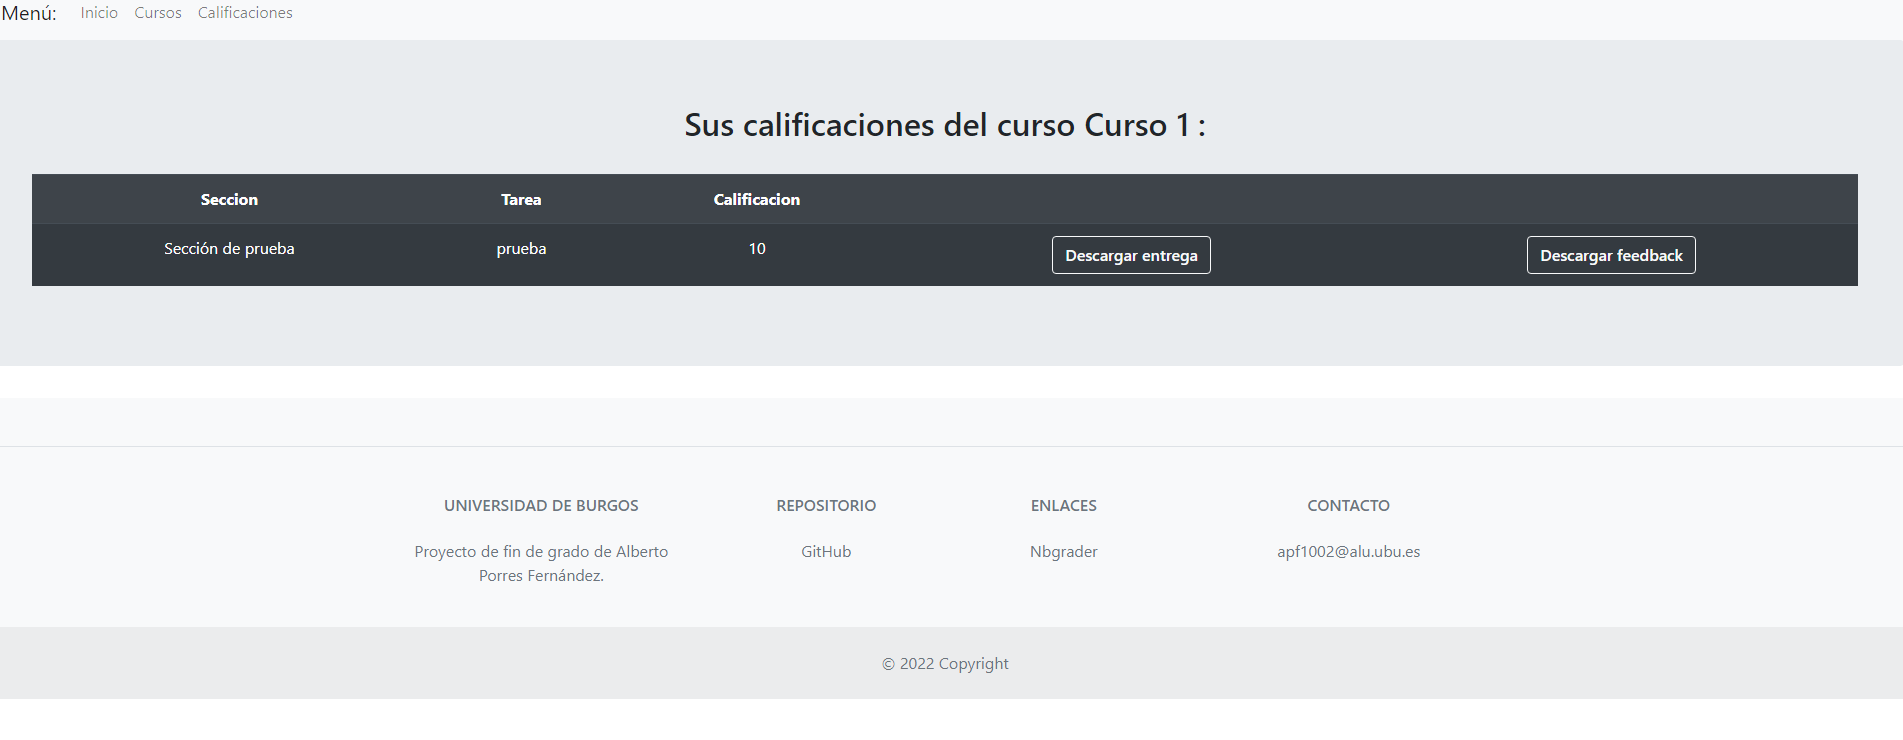
\includegraphics[width=\textwidth]{img/imgs-memoria/CalificacionesCurso.PNG}
\caption{Página de Calificaciones del Curso}
\end{figure}

En esta página tendrá acceso a los documentos tarea entregados y feedback de cada calificación mediante el botón \textbf{Descargar entrega} y \textbf{Descargar feedback}.


\subsection{4 Resolución de tareas}
La resolución de tareas debe realizarse mediante la herramienta Jupyter Notebooks la cual el alumno tiene que tener instalada en su ordenador de trabajo.


\subsection{5 Consulta de todas las calificaciones}
Para consultar todas las calificaciones obtenidas ha de hacer click en el botón \textbf{Ir a mis calificaciones} de la \textbf{Página principal del alumno}(\ref{PagAlumno}) o haciendo click en el botón \textbf{Calificaciones} de la barra navegacional superior. Esto le llevará a la \textbf{Página de calificaciones global}:

\begin{figure}[H]
\centering
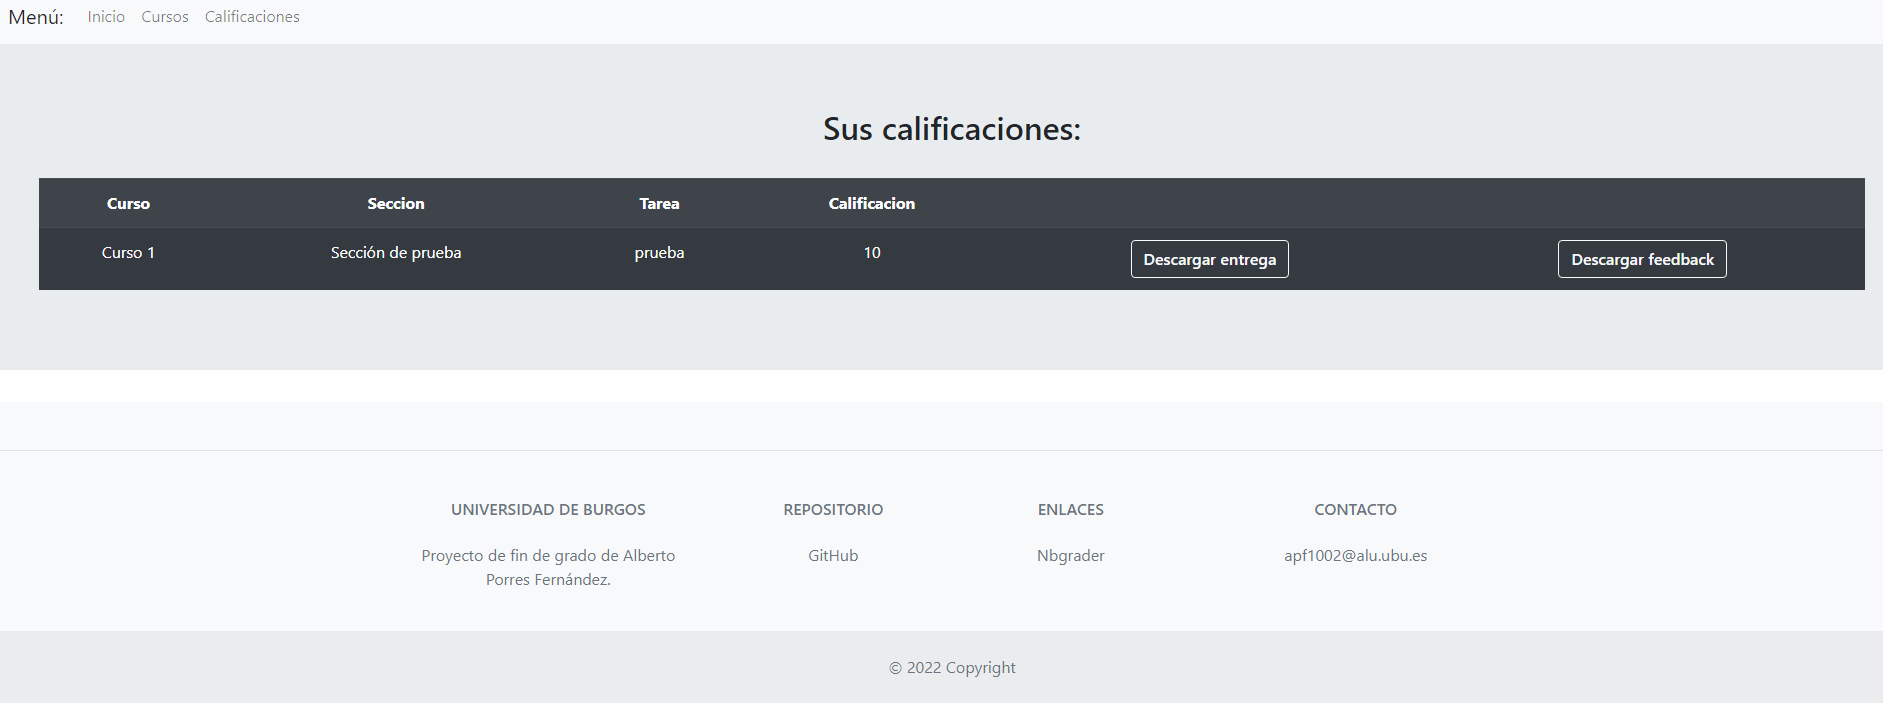
\includegraphics[width=\textwidth]{img/imgs-memoria/CalificacionesAlumno.PNG}
\caption{Página de Calificaciones Global del alumno}
\end{figure}

Desde esta también tendrá acceso a los documentos de entrega y feedback mediante los respectivos botones.



\subsection{6 Cambio de contraseña}
Para acceder al cambio de contraseña de su cuenta se ha de hacer click en el botón \textbf{Cambiar Contraseña} de la \textbf{Página principal del alumno}\ref{PagAlumno}. Esto le llevará al formulario de cambio de contraseña:

\begin{figure}[H]
\centering
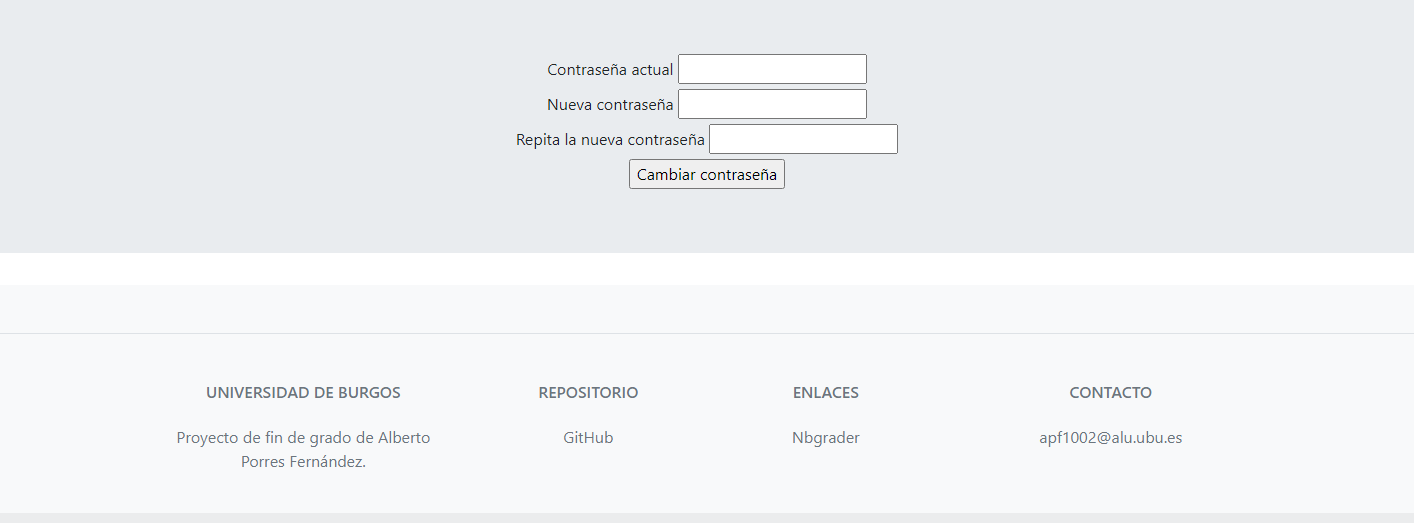
\includegraphics[width=\textwidth]{img/imgs-memoria/CambiarContra.PNG}
\caption{Página de cambio de contraseña del alumno}
\end{figure}

Al completar el formulario y aceptar el modal de confirmación emergente, su sesión será cerrada siendo redireccionado al login.

\subsection{7 Cierre de sesión} 
El cierre de sesión se realiza haciendo click en el botón \textbf{Cerrar Sesión} de la \textbf{Página principal del alumno}(\ref{PagAlumno}) y aceptando el modal de confirmación emergente.
